%%%%%%%%%%%%%%%%%%%%%%% file typeinst.tex %%%%%%%%%%%%%%%%%%%%%%%%%
%
% This is the LaTeX source for the instructions to authors using
% the LaTeX document class 'llncs.cls' for contributions to 
% the Lecture Notes in Computer Sciences series.
% http://www.springer.com/lncs       Springer Heidelberg 2006/05/04
%
% It may be used as a template for your own input - copy it 
% to a new file with a new name and use it as the basis
% for your article. 
%
%%%%%%%%%%%%%%%%%%%%%%%%%%%%%%%%%%%%%%%%%%%%%%%%%%%%%%%%%%%%%%%%%%%


\documentclass[runningheads]{llncs}

\usepackage{amssymb}
\setcounter{tocdepth}{3}
\usepackage{graphicx}
\graphicspath{{../figures/}}

\usepackage{algorithm}
\usepackage{algorithmic}
\usepackage{tabularx}
\usepackage{multirow}
\usepackage{rotating}
\usepackage{comment}


\usepackage[latin1]{inputenc}
\usepackage{url}
\usepackage{epsf}
\urldef{\mailsa}\path|kartik@ee.iitb.ac.in|
\urldef{\mailsb}\path|gabriel.caffarena@ceu.es|
\urldef{\mailsc}\path|alberto.gilf@gmail.com|
\urldef{\mailsd}\path|david.gonzalez.marquez@usc.es|
\urldef{\mailse}\path|abraham.otero@gmail.com|
\urldef{\mailsf}\path|madhav@ee.iitb.ac.in|
\newcommand{\keywords}[1]{\par\addvspace\baselineskip
\noindent\keywordname\enspace\ignorespaces#1}


\def\NoNumber#1{{\def\alglinenumber##1{}\State #1}\addtocounter{ALG@line}{-1}}

\begin{document}

\mainmatter  % start of an individual contribution

% first the title is needed
\title{Low-latency Hermite Polynomial Characterization of Heartbeats using a Field-Programmable Gate Array}

% a short form should be given in case it is too long for the running head 
\titlerunning{Low-latency Hermite Polynomial Characterization using an FPGA}


% the name(s) of the author(s) follow(s) next
%
% NB: Chinese authors should write their first names(s) in front of
% their surnames. This ensures that the names appear correctly in
% the running heads and the author index.
%
\author{Kartik Lakhotia\inst{1} \and
 Gabriel Caffarena\inst{2} \and 
 Alberto Gil\inst{3} \and
 David G. Marquez \inst{3} \and 
 Abraham Otero\inst{2} \and
 Madhav P. Desai \inst{1}}

% if the list of authors exceeds the space for a headline,
% an abbreviated author list is needed
\authorrunning{Kartik Lakhotia et al.}
% (feature abused for this document to repeat the title also on left hand pages)



% the affiliations are given next
\institute{Indian Institute of Technology (Bombay), \\
Powai, Mumbai 400076, \\
India\\
\mailsa\\
\mailsf\\
\and 
University CEU-San Pablo,\\
Urb. Monteprincipe, 28668, Madrid, Spain\\
\mailsb\\
\mailsc\\
\mailsd\\
\mailse\\
\and
Centro Singular de Investigacion en Tecnologias da Informacion (CITIUS),\\
University of Santiago de Compostela, 15782 Santiago de Compostela, Spain
}

%
% NB: a more complex sample for affiliations and the mapping to the
% corresponding authors can be found in the file "llncs.dem" 
% (search for the string "\mainmatter" where a contribution starts).
% "llncs.dem" accompanies the document class "llncs.cls".
%
\toctitle{Lecture Notes in Computer Science}
\tocauthor{Authors' Instructions}
\maketitle


\begin{abstract}
The characterization of ECG heartbeats is a computationally intensive problem, and
both off-line and on-line (real-time) solutions to this problem are of great interest.
In this paper, we consider the use of a dedicated hardware implementation
(using a field-programmable gate-array (FPGA)) to solve a critical component of this problem. 
We describe an implementation of real-time best-fit Hermite approximation of a heartbeat using six Hermite polynomials.  
The implementation is generated using an algorithm-to-hardware compiler tool-chain
and the resulting hardware is characterized using an off-the-shelf FPGA card.
The single beat best-fit computation latency is under $0.5ms$ with a power dissipation of 3 watts.

\keywords{Hermite approximation, ECG, QRS, Arrhythmia,  FPGA, Parallelization}
\end{abstract}


\section{Introduction}

Automatic ECG analysis and characterization can be of great help
in patient monitoring.
In particular, the characterization of the QRS complex by means of Hermite functions 
seems to be a reliable mechanism  for automatic classification of heartbeats \cite{j:lagerholm00}. 
The main advantages seem to be the low sensitivity to noise and artifacts, and the
compactness of the representation (e.g. a 144-sample QRS can be characterized with 7 parameters \cite{c:marquez13}). 
These advantages have made the Hermite representation a very common tool for characterizing the 
morphology of the beats \cite{j:lagerholm00,c:marquez13,c:braccini97,j:linh03a,j:linh03b}. 

ECG analysis using Hermite functions has a
substantial amount of parallelism.  Solutions to the problem have been investigated
using processors (and multi-cores) and graphics processing units (GPU's). 
In this paper, we consider the alternative route of using an FPGA to implement
the computations.  In particular, our work is motivated by the potential
of an FPGA (or eventually, a dedicated application-specific circuit) for low-latency
energy efficient heart-beat analysis.  

In generating the hardware for heart-beat analysis, we make extensive use of
algorithm-to-hardware techniques.  By this we mean that the hardware is
generated from an algorithmic specification that is written in a
high-level programming language ({\bf C} in this case), which is then
transformed to a circuit implementation using the AHIRV2 algorithm to hardware 
compilation tools \cite{c:ahir_thesis2009,c:ahir_dsd2010,c:ahir_usenix2012}.
The resulting hardware is then mapped to an FPGA card (the ML605 card from Xilinx,
which uses a Virtex-6 FPGA).  The circuit is then exercised through the PCI-express 
interface and used to classify beats.  The round-trip latency of a single
beat classification was found to be under $0.5ms$.


\section{QRS approximation by means of Hermite polynomials}\label{s:arr}

The aim of using the Hermite approximation to estimate heartbeats is to 
reduce the number of dimensions required to carry out the ECG classification, 
without sacrificing accuracy. 
The benchmarks used in this work come from the MIT-BIH arrhythmia database \cite{j:moody01} which is made up of 
48 ECG recordings whose beats  have been manually annotated by two cardiologists. 
Each file from the database 
contains 2 ECG channels, sampled at a frequency of 360 Hz and with a duration of approximately 2000 beats. 

Before doing the Hermite approximation, the ECG signal is processed to remove
the base-line drift.  The QRS complexes for each heartbeat are extracted by 
finding the peak of the beat (e.g. the R wave) and selecting a  window of 200 ms centered on the peak. 
The beat-window is further extended to 400 ms by padding 100-ms sequences of zeros at each side of the complex. 
Thus, the QRS beat data used as an input to the Hermite polynomial approximation
consists of individual beats described as a 144-sample vector $\vec{x}=\{x(t)\}$ of double
precision floating point numbers. 
This vector is to be estimated with a linear combination of $N$ Hermite basis functions (for
the work reported in this paper, we use $N=6$).

The goal then is to find the best minimum-mean-square-error (MMSE)  approximation to
$\{ x(t)\}$ as 
\begin{equation}\label{eqn:hat}
\hat{x}(t)=\sum_{n=0}^{N-1}c_n(\sigma )\phi_n(t,\sigma),
\end{equation}

\noindent with

\begin{equation}\label{eqn:phi}
\phi_n(t,\sigma )=\frac{1}{\sqrt{\sigma 2^n n!\sqrt{\pi}}}e^{-t^2/2\sigma^2}H_n(t/\sigma) 
\end{equation}

\noindent where $H_n(t/\sigma)$ is the $n^{th}$ Hermite polynomial. 
These polynomials can be computed recursively as

\begin{equation}
H_n(x)=2xH_{n-1}(x)-2(n-1)H_{n-2}(x),
\end{equation}

\noindent where $H_0(x)=1$ and $H_1(x)=2x$.
The parameter $\sigma$ controls the width of the polynomials. In \cite{j:lagerholm00} the maximum value 
of $\sigma$ for a given order $n$ is estimated.  As the value of $n$ increases, the value of $\sigma_{MAX}$ decreases.

The Hermite polynomials are orthornormal.  Thus, the optimal coefficients that 
minimize the estimation error for a given $\sigma$ are

\begin{equation}\label{eqn:c}
c_n(\sigma)=\sum_{t} x(t)\cdot \phi_n(t,\sigma) 
\end{equation}

The best fit is calculated by comparing the MMSE approximation for each $\sigma$, and keeping
the one with the smallest value.
Once the best $\sigma$ and the corresponding fit coefficients $\vec{c}=\{c_n(\sigma)\}$  \mbox{$(n\in [0,N-1])$} 
are found for each heartbeat, it is possible to use only these figures to perform morphological 
classification of the heartbeats \textrm{~\cite{j:lagerholm00}}.

\section{Beginning the FPGA implementation: the algorithm} \label{s:algorithm}

The algorithm used in the FPGA implementation is illustrated in 
Figure \ref{fig:FpgaAlgo}.
\begin{figure}
\begin{centering}
\begin{verbatim}
void HermiteBestFit()
{  
    receiveHermiteBasisFunctions();

    while(1)
    {
        receiveHeartBeat();
        innerProducts();
        findBestFit();
        reportResults();
    }
}
\end{verbatim}
\end{centering}
\caption{High-level view of algorithm mapped to the FPGA}
\label{fig:FpgaAlgo}
\end{figure}

The implementation first receives the values of the Hermite polynomial basis
functions, and  stores them in distinct arrays in the hardware.  In the
current implementation, we use six
arrays to store the basis functions for order $n=0$ to $n=5$.  For each
$n$, basis functions for ten different values of $\sigma$ are stored in the corresponding
array.  The values of $\sigma$ used range from $1/120$ to $1/90$.

After this initialization step, the hardware executes a continuous loop.  
In the loop body, the hardware first listens for heart beats. When
a complete heart-beat (144 samples) is received, the inner products of the
heart-beat with all the basis functions are calculated in a double loop.  
After all inner products are calculated, the inner product coefficients
are used to compute the best fit among the different values of $\sigma$.
The best-fit $\sigma$ index and the fitted values are then written
out of the hardware.

The algorithm as described above is purely sequential
and does not contain any explicit parallelization.  The AHIRV2 compiler
is intelligent enough to extract parallelism from the two critical
loops (in the inner-product and best-fit functions).

Even with this simple coding of the hardware algorithm,
we observe that excellent real-time performance
is observed (in comparison with CPU/GPU implementations).
Going further, it is possible to specify explicit parallelism by
and exploit it by using multiple function units in hardware
in order to reduce the processing latency.  These investigations
are currently in progress.



\subsection{The inner product loop} \label{sec:InnerProduct}

\begin{figure}
\begin{centering}
\begin{verbatim}
void  innerProduct()
{
  int I;
  for (I=0; I < NSAMPLES; I++)
  { // outer-loop
     double x = inputData[I];
     for(SI = 0; SI < NSIGMAS; SI++)
     { // inner-loop
        int I0 = I + Offset[SI];
        double p0 = (x0*hF0[I0]);
        double p1 = (x0*hF1[I0]);
        double p2 = (x0*hF2[I0]);
        double p3 = (x0*hF3[I0]);
        double p4 = (x0*hF4[I0]);
        double p5 = (x0*hF5[I0]);
        dotP0[SI] += p0;
        dotP1[SI] += p1;
        dotP2[SI] += p2;
        dotP3[SI] += p3;
        dotP4[SI] += p4;
        dotP5[SI] += p5;
     }
}
\end{verbatim}
\end{centering}
\caption{Inner-product loop}
\label{fig:InnerProduct}
\end{figure}

The inner product loop is shown in Figure \ref{fig:InnerProduct}.
The outer loop is over the samples, and the inner
loop across the $\sigma$ values.  There is a high-level
of parallelism in the inner loop which can be further
boosted by unrolling the outer loop.   When translating
this to hardware, the entire function uses one single double-precision
multiplier and one single double-precision adder.  Further
note that the arrays $hFn$ and $dotPn$ are declared on
a per-$n$ basis (for $n=0$ to $n=5$). This allows the arrays to be mapped to
distinct memory spaces, thus increasing the memory access bandwidth in the hardware.

\subsection{The minimum-mean-square loop} \label{sec:MMSE}

\begin{figure}
\begin{centering}
\begin{verbatim}
void computeMSE()
{
  int I, SI;
  best_mse = 1.0e+20;
  best_sigma_index = -1;
  for (I=0; I<NSAMPLES; I=I+4)
  { // outer-loop
     for (SI=0; SI<NSIGMAS; SI++)
     { // inner-loop
        int fetchIndex0 = I + Offset[SI]; 
        double p0 = (dotP0[SI]*hF0[fetchIndex0]);
        double p1 = (dotP1[SI]*hF1[fetchIndex0]);
        double p2 = (dotP2[SI]*hF2[fetchIndex0]);
        double p3 = (dotP3[SI]*hF3[fetchIndex0]);
        double p4 = (dotP4[SI]*hF4[fetchIndex0]);
        double p5 = (dotP5[SI]*hF5[fetchIndex0]);
        double diff = (inputData[I]-
                         ((p0+p1) + (p2+p3) + (p4+p5)));
        err[SI] += (diff*diff);
      }
    }
    for (SI=0; SI<NSIGMAS; SI++)
    {
        if(err[SI] <  best_mse)
        {
           best_mse = err[SI];
           best_sigma_index = SI;
        }
    }
}
\end{verbatim}
\end{centering}
\caption{MMSE calculation loop}
\label{fig:MMSE}
\end{figure}


The MMSE calculation hardware
uses the algorithm shown in Figure \ref{fig:MMSE}.
Note that the inner loop again has considerable parallelism.
One pipelined double precision multiplier and one
pipelined double precision adder are used to implement
the loop.  The arrays referred to in the loop
$dotPn$ and $hFn$ are all implemented in disjoint
memories to give high memory access bandwidth.



\subsection{Further optimizations}

The current implementation uses a simple sequential specification.
We have investigated the impact of
further optimizations.  In particular, we find that outer-loop
unrolling (up to four) and inner-loop pipelining 
have substantial impact on the performance of the generated hardware.
This data is reported in Section \ref{s:results}.

\section{Hardware Implementation Details}\label{s:implementation}

The overall system has 3 major components:
\begin{itemize}
\item A host computer, which is used to calculate the Hermite basis functions,
initialize the FPGA card, send beat data to the FPGA card and receive
the best-fit coefficients from the FPGA card.
\item The FPGA card, on which the best-fit algorithm is implemented.   We use the
Xilinx ML605 card which features a Virtex-6 FPGA and an 8-lane PCI express interface.
\item The FPGA card driver, which is based on the RIFFA infrastructure \cite{c:jacobsen13}. 
\end{itemize}

The algorithm mapped to the FPGA 
is first described in a C program (code fragments descibed in Sections \ref{s:algorithm},  \ref{sec:InnerProduct} and \ref{sec:MMSE}).
The architecture of the hardware produced is shown in Figure \ref{fig:HardwareArchitecture}.
In the initialization phase, the hardware-side listens on an input FIFO to acquire
the Hermite polynomials (these are stored in six disjoint memories, one
for each order $n=0,1,2,\ldots 5$).  After this step, the unit that receives
the beat samples is triggered.  This unit listens on the input FIFO and receives a 144 sample
heartbeat (coded as 144 double-precision floating point numbers).  After receiving
the sample, it triggers the inner-product stage.  In the inner-product stage, the hardware computes, for each $\sigma$ and
$n$, an inner product of the received beat with the Hermite polynomials $\phi_n(t,\sigma)$.
We are using ten values of $\sigma$ and $6$ values of $n$.  Thus, 60 inner-products
are computed in this phase.  The inner products are stored in ten
disjoint memories, one for each $\sigma$.  After this is done, the MMSE
stage is triggered.  In the MMSE stage, the inner-products are used to find the best fit $\sigma$.
The computed best-fit coefficients are sent back to the host using the output FIFO.
The hardware unit which listens for the next beat is then triggered (wait for the next beat).

\begin{figure}
\begin{center}
	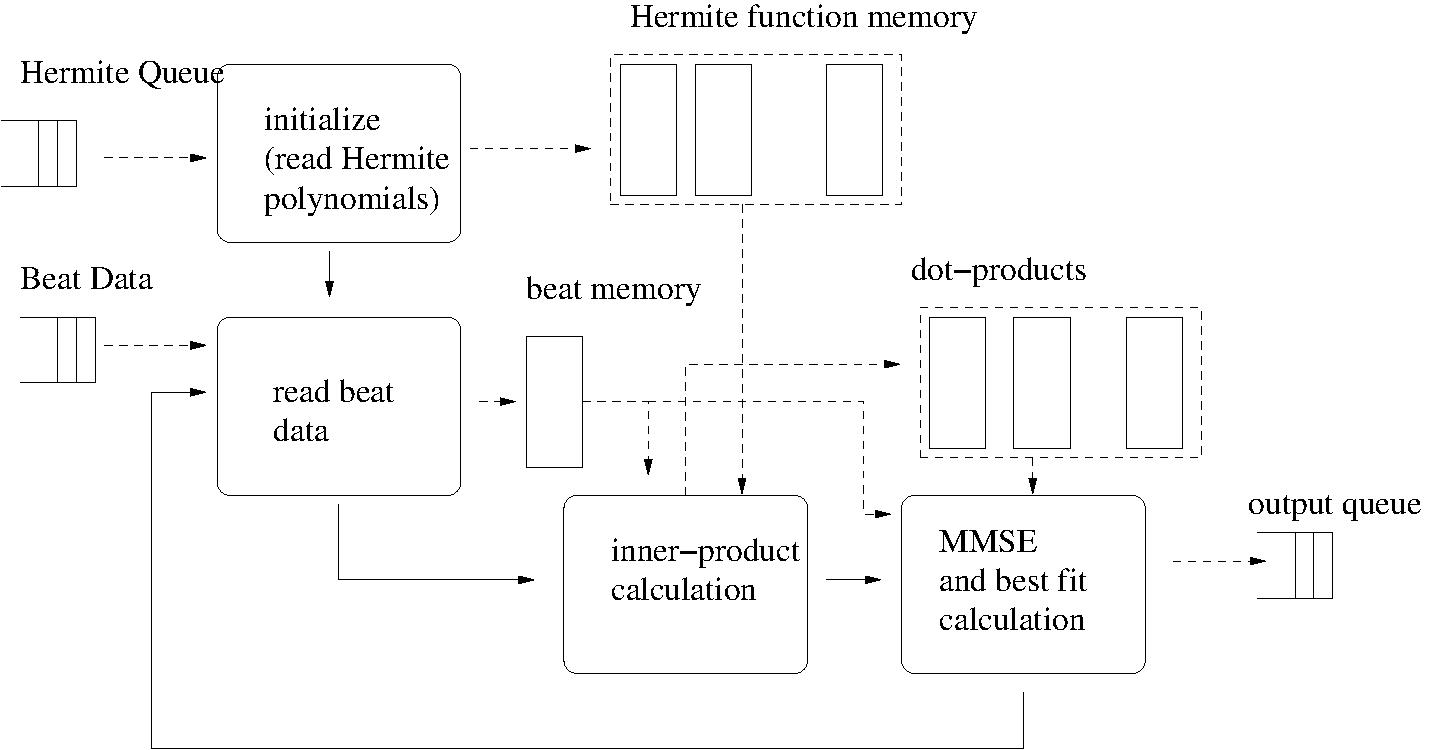
\includegraphics[scale=0.50]{HardwareArchitecture.pdf}
	\caption{Hardware Architecture}
	\label{fig:HardwareArchitecture}
\end{center}
\end{figure}

The VHDL hardware for this design is generated using AHIR-V2 toolchain \cite{c:ahir_usenix2012}.  
The generated VHDL is instantiated in the FPGA together with the RIFFA wrappers,
and the resulting design is synthesized and mapped to the Virtex-6 FPGA using
the Xilinx ISE 14.3 toolset.


%
%HDL for this design is generated using AHIR HLS toolchain. It is equipped with a library 
%of heavily pipelined Floating Point operators and Loop Pipelining mechanism which 
%enables the final VHDL to extract parallelism in C program. It uses pipes to communicate 
%between testbench and the program, which translate to FIFOs in hardware. A simple integration 
%interface between these FIFOs and RIFFA channels completes the system. 
%
%
%The RIFFA software drivers and interface infrastructure is used to communicate between 
%host and FPGA card \cite{c:jacobsen13}. It supports upto 12 independent
%channels for data transmission. All of them end in separate Rx/Tx FIFOs on FPGA that 
%can operate on different clock domains at either ends. A simple integration 
%interface bridges RIFFA and AHIR generated FIFOs.
%By incorporating functions provided by RIFFA driver, same testbench used for 
%Software verification can be used for verifying the hardware.
%  Describe the 
%    - overall system.
%    - card
%    - the driver
%    - the hardware generation process.
%
\section{Results}\label{s:results}

We measure the round-trip delay and FPGA core power consumption for processing one beat. 
The round-trip delay is the time interval between the beginning of transmission of 
beat-data from the host to the hardware and the beginning of reception of best fit
coefficients from the hardware. 
The test feeds a single beat at a time to the FPGA and measures the latency.

In the implementation, the two outer-loops described in Sections \ref{sec:InnerProduct} and
 \ref{sec:MMSE} were unrolled to different
extents to see the impact of unrolling on the system performance. 
Three levels of unrolling were tried: one-way, two-way and four-way.  
The four-way unrolling gave the best performance,
as expected.  The results are summarized in Table \ref{table:Results} (the reported latency
is the average value observed across 100 beats).  
The minimum latency achieved with four-way-unrolling was observed to be
$0.39$ ms (for the processing of a single 144-sample beat).
The power dissipation values are
measured using hardware monitoring while the beats are being processed, and represent peak
power dissipation.

%%%%%%%% Results Table %%%%%%%%%%%%%
\begin{table}[ht]
\caption{Results:  FPGA utilization and latency for different loop-unrolling levels} %title
\centering
\begin{tabular}{c @{\hskip 0.06in}| @{\hskip 0.06in}c@{\hskip 0.2in}c @{\hskip 0.2in} c @{\hskip 0.2in} c} %5 centered columns
\hline\hline\\[-1.5ex]

Unroll-level & \begin{tabular}[c]{@{}c@{}}Slice LUT  \\ Utilization  \end{tabular}& \begin{tabular}[c]{@{}c@{}}Slice Register  \\Utilization  \end{tabular}& \begin{tabular}[c]{@{}c@{}}Avg. Processing  \\Latency \end{tabular} & \begin{tabular}[c]{@{}c@{}}FPGA core Power \\ Consumption \end{tabular}\\ [2ex] \hline \\[-1.5ex]%heading

1-way & 56839 & 65995 & 1.39ms & 2.75W \\

2-way & 65895 & 80709 & 0.80ms & 2.88W \\

4-way & 84331 & 110165 & 0.44ms & 3.09W \\ [1ex]

\hline
\end{tabular}
\label{table:Results}
\end{table}
%%%%%%%%%%%%%%%%%%%%%%%%%%%

It is clear that FPGA can be used for real-time processing since the 
computation time required to process a pair of beats (corresponding
to a heart-beat sampled on two channels) is less than $1ms$, which is
much smaller than time-interval between actual heart beats (which is about $1s$). 
The observed power dissipation is 3.1W.  Hardware utilization in 4-way unrolled 
system is less than $55\%$ of the FPGA resource.

\subsection{Comparison with GPU/CPU implementations}

Hermite basis fitting has been evaluated on GPU and CPU implementations
as well.  For example, in \cite{c:GPU}, the authors demonstrate a
GPU implementation that shows excellent scaling behaviour, so that 
100K beats can be processed in 15.7 seconds.  However, when it comes
to the latency needed to process a pair of beats, the FPGA can
process a beat-pair in under $1ms$, whereas the CPU and GPU implementations
can process a single beat-pair in $15ms$ and $5ms$ respectively.
Thus, the FPGA beat-pair processing latency shows a 15X improvement relative to
the CPU and a 5X improvement relative to the GPU. 
These comparisons are made against same algorithm executed on Intel-i7 PC(1.6GHz) 
and NVIDIA TESLA C2050 (1.15GHz) \cite{c:GPU}. The operating frequency on the FPGA
card was 100MHz which is less than one-tenth of that used on CPUs and GPUs.
Further, the peak power consumption (while actually processing the beats) on the FPGA is 3W as compared to $100W+$ on Core i7 processors and
$200W+$ on the GPU.  %% which GPU?
Thus, the FPGA is an attractive option for low energy real-time ECG classification
applications in portable health monitoring devices.

\section{Conclusions}\label{s:conclusions}

In this paper, a solution to the problem of Hermite polynomial
based heart-beat characterization using FPGAs is presented.
We have mapped the problem to hardware using algorithm-to-hardware
techniques (with the AHIRV2 tools).  The Xilinx ML605 card with a
Virtex-6 FPGA was used as the platform and the RIFFA host-interface was used to
communicate with the FPGA card. 

This methodology is presented as an alternative to existing software oriented approaches, 
for real-time latency-sensitive signal processing. When using the FPGA, a substantial
latency reduction in single-beat processing was observed (in comparison with both
GPU and CPU implementations of the same algorithm).  
Further, the peak power dissipation in
the FPGA is almost two orders of magnitude lower than that observed in the CPU/GPU case.

The highly parallel GPU and CPU architectures are very effective in off-line processing
(processing of a large number of beats, not necessarily in real-time).  When it comes to real-time,
online beat processing, our work demonstrates that dedicated hardware implementation
using an FPGA offers a very competitive platform for ECG signal processing.

%%%% Couple of lines on Future work %%%%
 
% Bibliography
\bibliographystyle{splncs}
\bibliography{refsQRS}

\end{document}
